\section{Analisi Dati}
\subsection{Analisi degli Spettri}\label{sez analisi dati calibrazione}
Per calibrare in energia il \textit{Multi-Channel-Analyzer} sono stati presi due spettri, uno con la sorgente sperimentale $\ch{^{22}Na}$ ed uno con una sorgente di $\ch{^{137}Cs}$ .
I dati istogrammati sono poi stati analizzati tramite \textit{ROOT}\footnote{Codice consultabile al seguente link: \url{https://gitfront.io/r/MicheleScattola/GaGvFGBPX4Vm/Misure-Nucleari/tree/Compton/}}. Attorno al picco di emissione viene eseguito un fit Gaussiano al quale è aggiunto un fondo lineare. Per ottimizzare la regione di spettro su cui effettuare il fit viene prima stimato all'interno del codice il picco e la \textit{FWHM} tramite i bin dell'istogramma. Si riesce dunque ad effettuare il fit gaussiano in un intervallo di $\pm 3 \sigma$ attorno al picco ed inizializzando i parametri di fit con le stime iniziali.

I dati estrapolati dagli spettri di $\mu$ e $\sigma$ sono stati utilizzati per effettuare la calibrazione lineare in energia dei canali MCA.
Per quanto riguarda gli errori sui valori teorici si è fatto riferimento al \textit{National Nuclear Data Center (NNDC)}\footnote{\url{https://www.nndc.bnl.gov/nudat3/}}; i dati completi sono riportati in appendice in tabella \ref{tab:ADC} . Si è dunque eseguito un fit (fig. \ref{fig:calibrazioneADC}) del tipo $y = ax + b$ ; i parametri sono poi stati utilizzati per convertire le successive misure da canali ADC ad energia.
\begin{figure}[H]
  \centering
  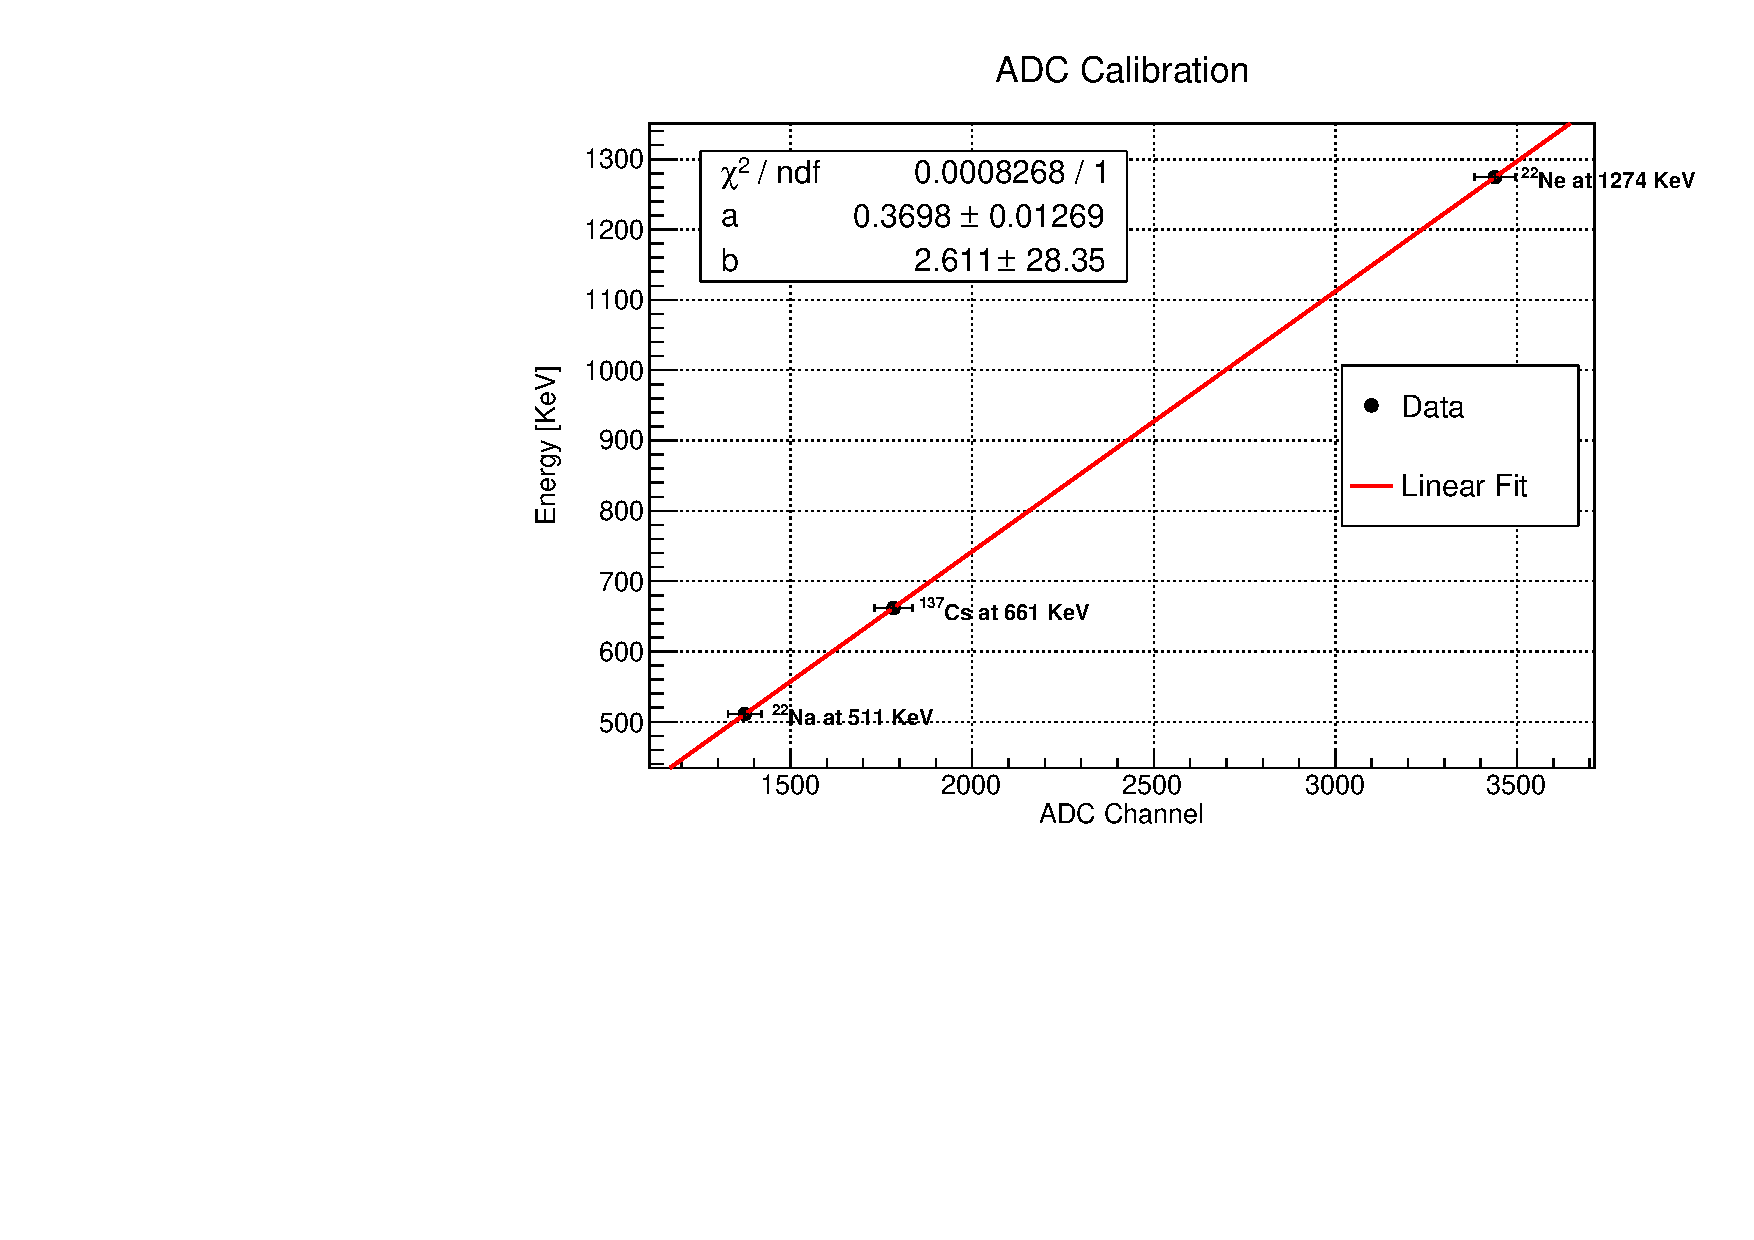
\includegraphics[scale=0.5]{Analisi Dati/linear.pdf} 
  \caption{Calibrazione ADC}
  \label{fig:calibrazioneADC}
\end{figure}
In seguito gli spettri acquisiti ai vari angoli $\theta$ sono stati analizzati in modo analogo al metodo utilizzato per la calibrazione, convertendo i canali ADC in Energia. L'analisi ha facilmente verificato lo spostamento del picco fotoelettrico; tutti gli spettri sono riportati in appendice \ref{appendice_spettri}, viene riportato in fig. \ref{fig:spettro60} quello ottenuto a 60 gradi.
\begin{figure}[H]
  \centering
  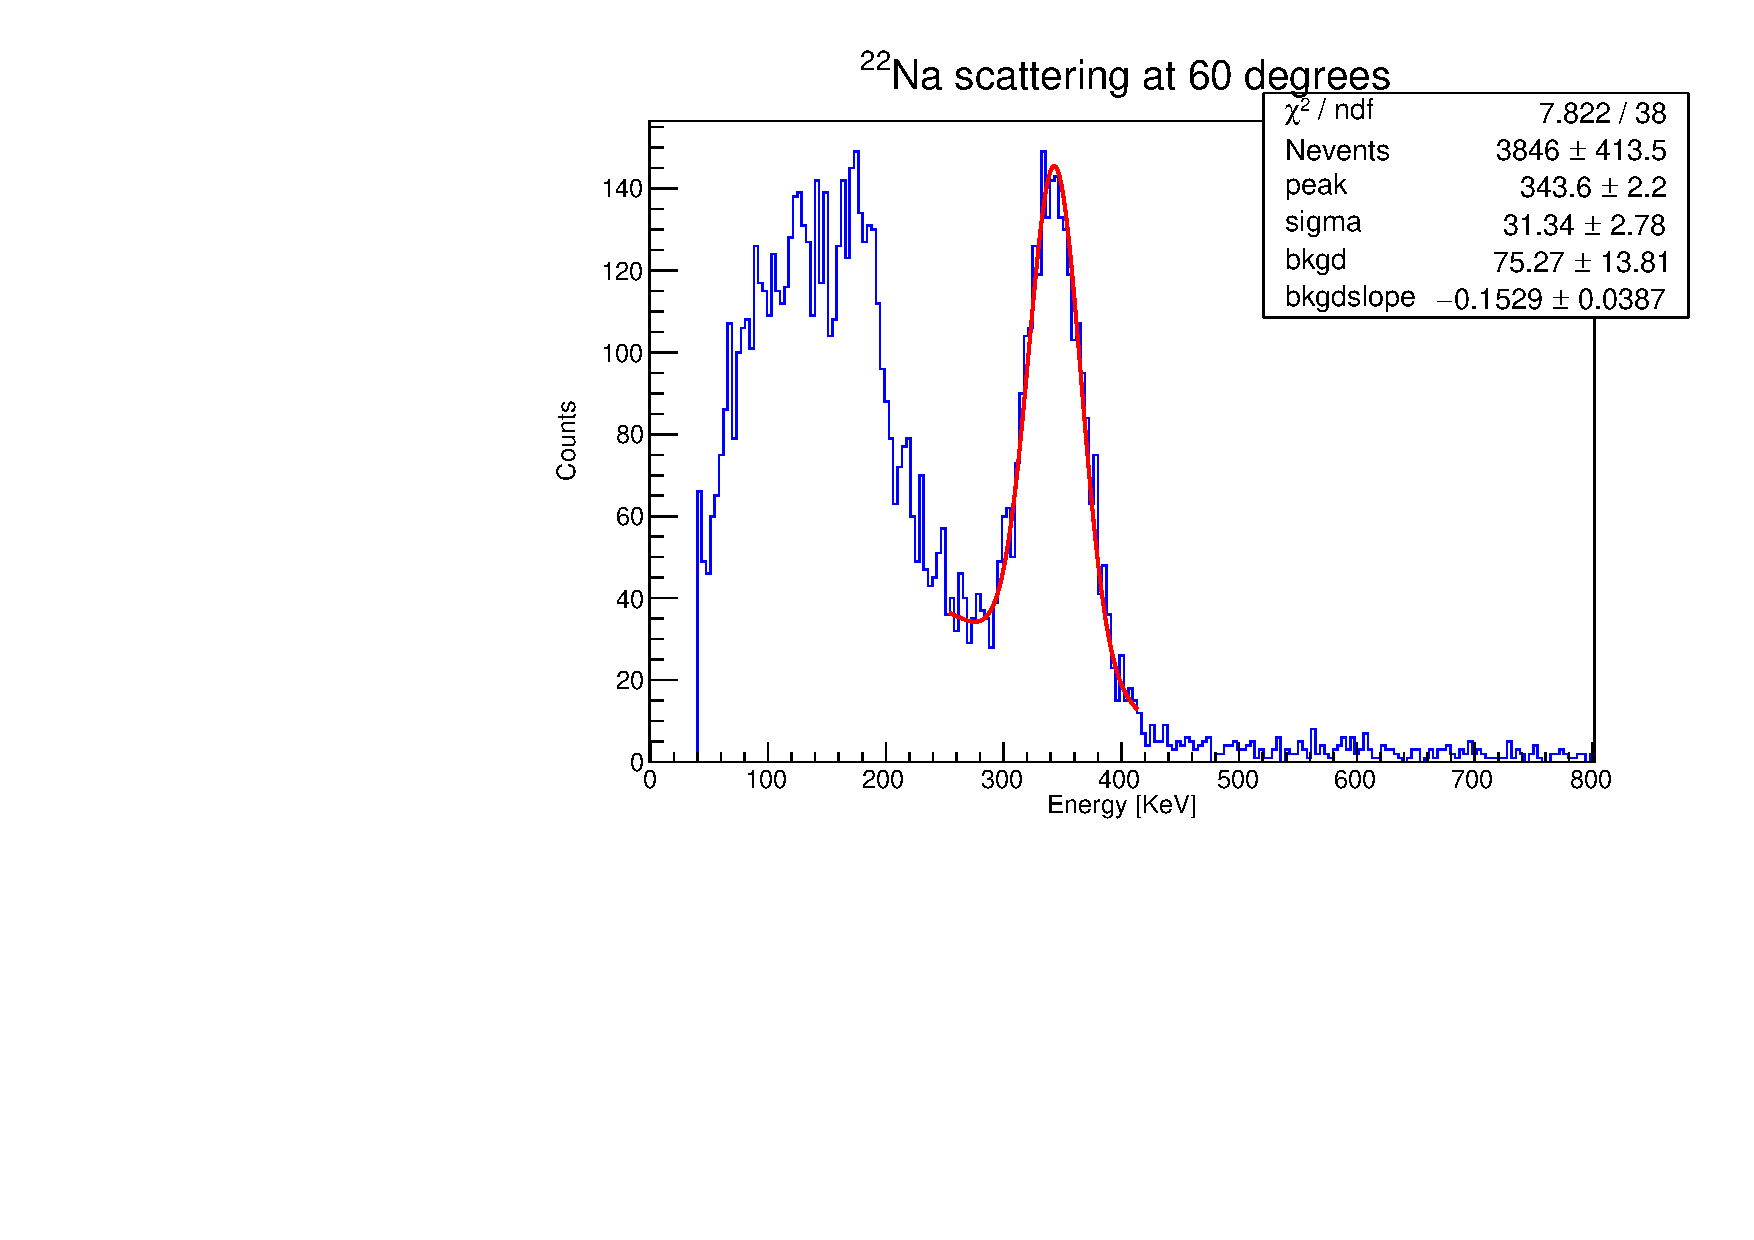
\includegraphics[scale=0.45]{Appendice/60_deg_spectrum.pdf} 
  \caption{Spettro acquisito a 60 gradi}
  \label{fig:spettro60}
\end{figure}
\subsection{Energia del fotone}
I dati estrapolati dagli spettri hanno permesso di rappresentare in fig. \ref{fig:E_gamma} l'energia del fotone uscente rispetto all'angolo di scattering - eq. \eqref{energia fotone uscente} . L'incertezza per i picchi è data da $\sigma_{TOT} = \frac{\sigma}{\sqrt{N}}$ dove N sono i conteggi sotto al picco e $\sigma$ la larghezza gaussiana. Queste incertezze risultano tuttavia considerevolmente minori rispetto a quelle relative alla posizione angolare e non sono dunque visibili nel grafico. I risultati completi sono disponibili in tabella in appendice \ref{tab:appendice_spettri}.
\begin{figure}[H]
  \centering
  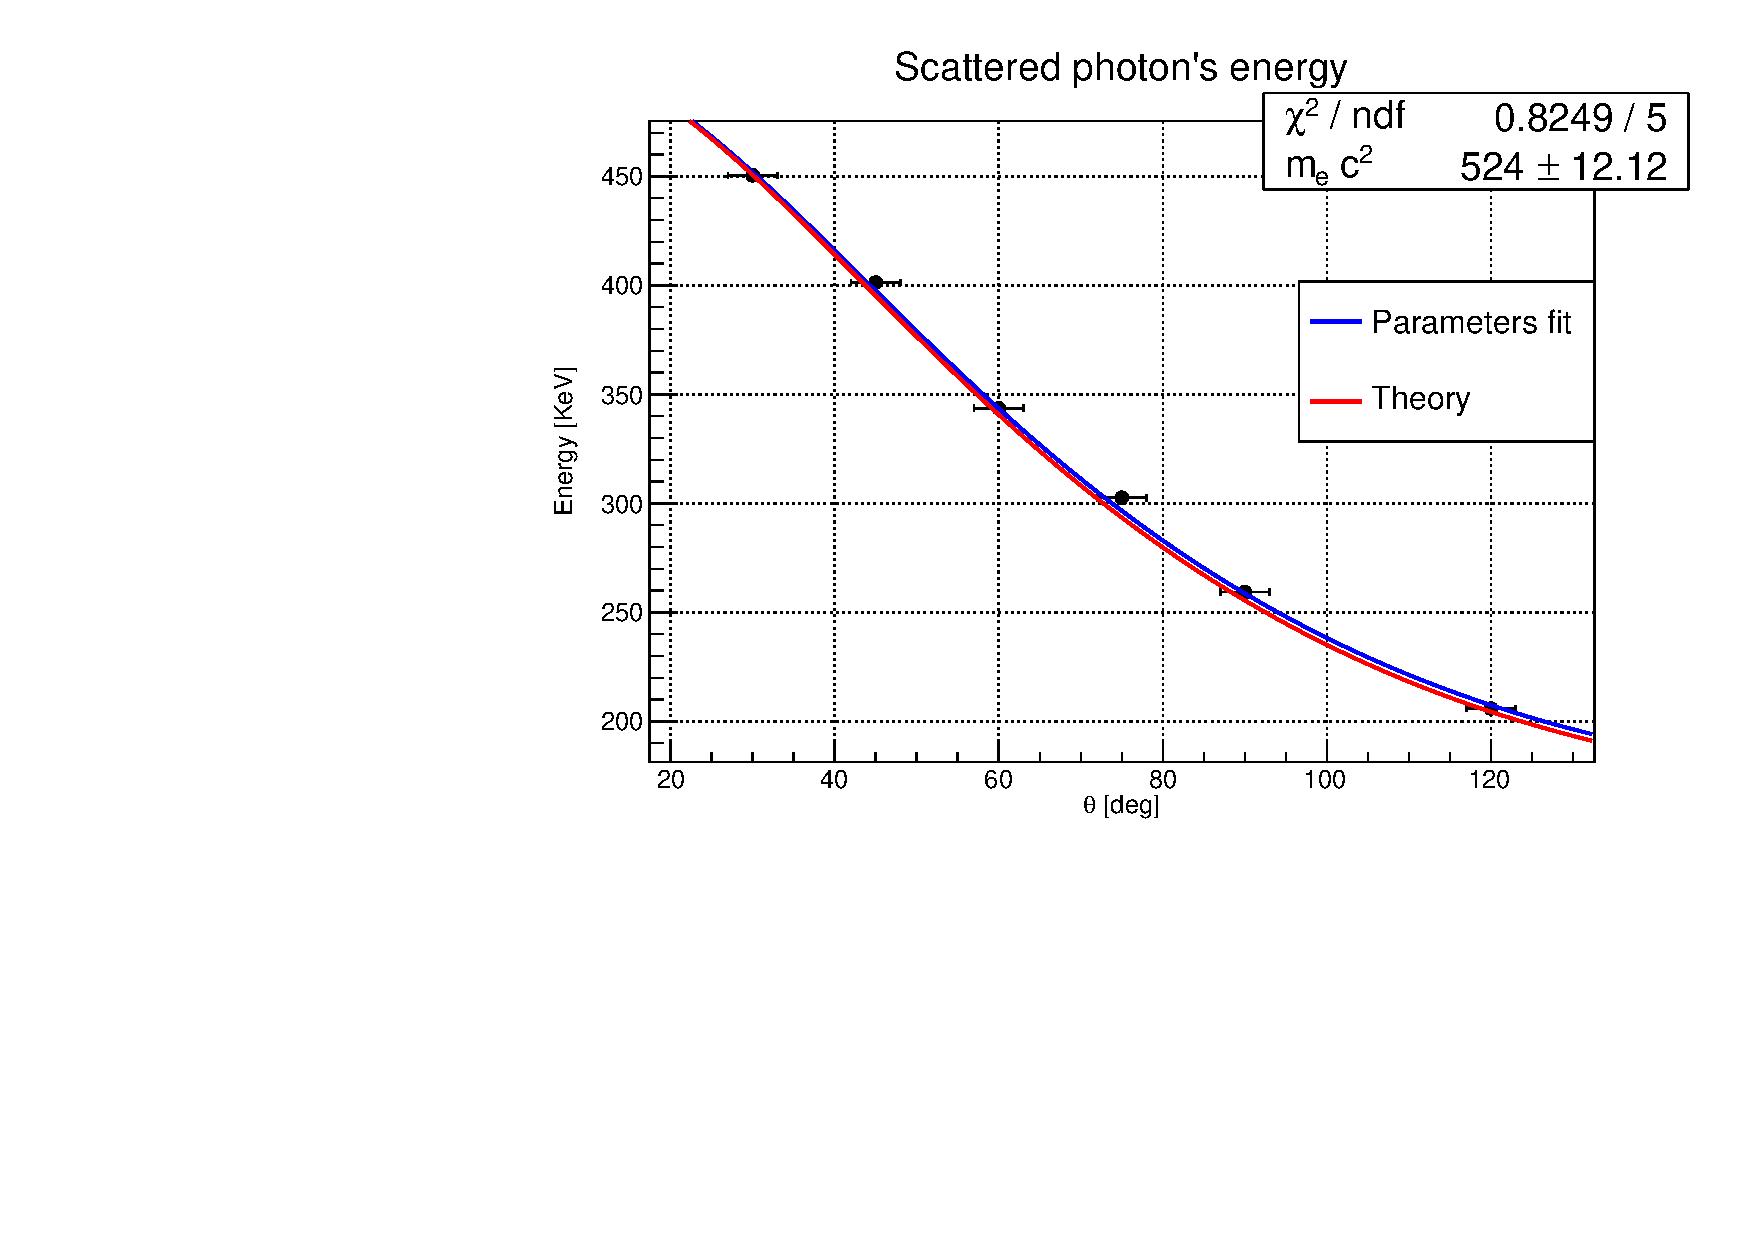
\includegraphics[scale=0.6]{Analisi Dati/E_1.pdf} 
  \caption{Ricostruzione della curva in energia del fotone uscente}
  \label{fig:E_gamma}
\end{figure}
Sono stati eseguiti due fit , i cui risultati sono riportati in tabella \ref{tab:risultati_energia}: il primo  relativo alla curva teorica ed il secondo lasciando come parametro libero il termine $m_e c^2$. Si nota inoltre che la curva parametrica si sovrappone a quella teorica confermando la bontà del risultato.
\begin{table}[H]
    \centering
    \begin{tabular}{|c c c c c|}
    \hline
    Tipo di fit & $\chi^2$ & $ndf$ & Probabilità  & $m_e c^2$ [\unit{\kilo\electronvolt}]\\ [0.5ex] 
 \hline\hline
 Teorico & 2.00 & 6 & 91.95 \% & 511 \\ 
 \hline
 Parametrico & 0.825 & 5 & 97.54 \% & $523\pm12$\\ 
 \hline 
    \end{tabular}
    \caption{Risultati di fit per l'energia del fotone uscente.}
    \label{tab:risultati_energia}
\end{table}
Si riferisce inoltre che lo spettro a 0 gradi è stato omesso dal grafico in seguito ad alcune considerazioni. Si notava infatti subito che fosse distaccato considerevolmente dal valore teorico ed avendo acquisito molti eventi vi è associata una incertezza molto piccola. Questo perchè la misura è stata effettuata alla fine dell'esperienza ad alcuni giorni di distanza da quelle precedenti e probabilmente le condizioni ambientali hanno modificato il comportamento sperimentale. Sarebbe stato dunque necessario effettuare una nuova calibrazione.
\subsection{Sezione d'urto}
Dalle misure sperimentali si è poi ricostruita la sezione d'urto data l'eq. \ref{eq sezione d'urto conteggi}. In seguito alle considerazioni in sezione \ref{sez_err_conteggi} le uniche misure utilizzabili per quanto riguarda i conteggi sono quelle a $30^\circ$, $45^\circ$, $60^\circ$ e $90^\circ$. L'errore associato alla misura è stato valutato tramite propagazione degli errori, la cui analisi viene affrontata in sezione \ref{sez_errori}. I dati ottenuti sono rappresentati in figura \ref{fig:sezione_sperimentale}.
\begin{figure}[H]
  \centering
  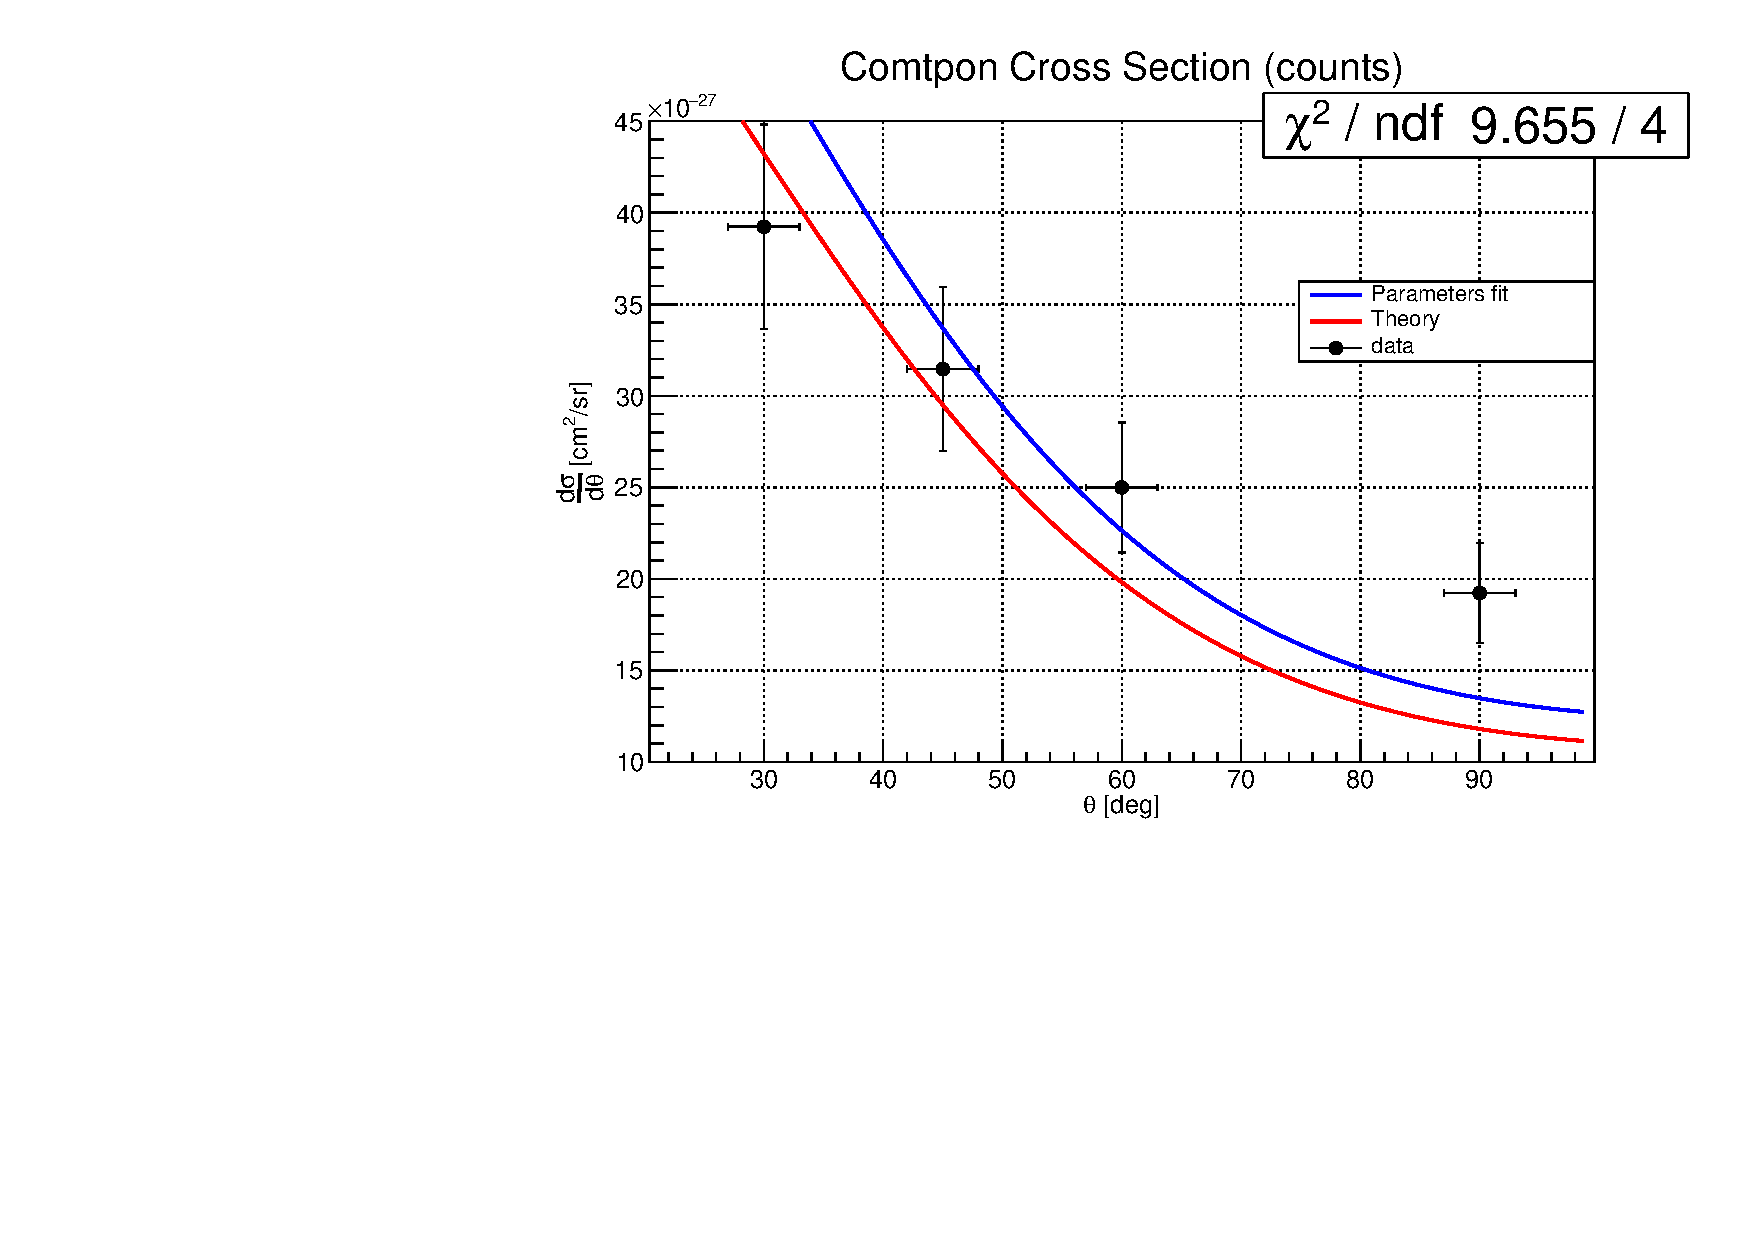
\includegraphics[scale=0.6]{Analisi Dati/ExpCrossSec_counts.pdf} 
  \caption{Ricostruzione della sezione d'urto Compton tramite i conteggi}
  \label{fig:sezione_sperimentale}
\end{figure}
Sui dati vengono eseguiti due fit analogamente a quanto fatto per l'energia del fotone uscente, i cui risultati sono disponibili in tabella \ref{tab:risultati_sezione}. In questo caso il parametro libero è il raggio classico dell'elettrone $r_e$.
\begin{table}[H]
    \centering
    \begin{tabular}{|c c c c c|}
    \hline
    Tipo di fit & $\chi^2$ & $ndf$ & Probabilità  & $r_e$ [fm]\\ [0.5ex] 
 \hline\hline
 Teorico & 9.65 & 4 & 4.76 \% & $\num{2.8179}$ \\ 
 \hline
 Parametrico & 7.31 & 3 & 6.27 \% & $\num{3.01}\pm\num{0.65}$\\ 
 \hline 
    \end{tabular}
    \caption{Risultati di fit per la sezione d'urto Compton.}
    \label{tab:risultati_sezione}
\end{table}

%Inoltre è stato possibile ricavare una stima della sezione d'urto tramite la formula di Klein-Nishina (\ref{eq sezione d'urto Klein-Nishina}) , utilizzando i picchi degli spettri acquisiti ai vari angoli. L'errore considerato proviene direttamente dalla propagazione degli errori visibile in appendice \ref{appendice_errore_sezione_energie}.
%\begin{figure}[H]
  %\centering
  %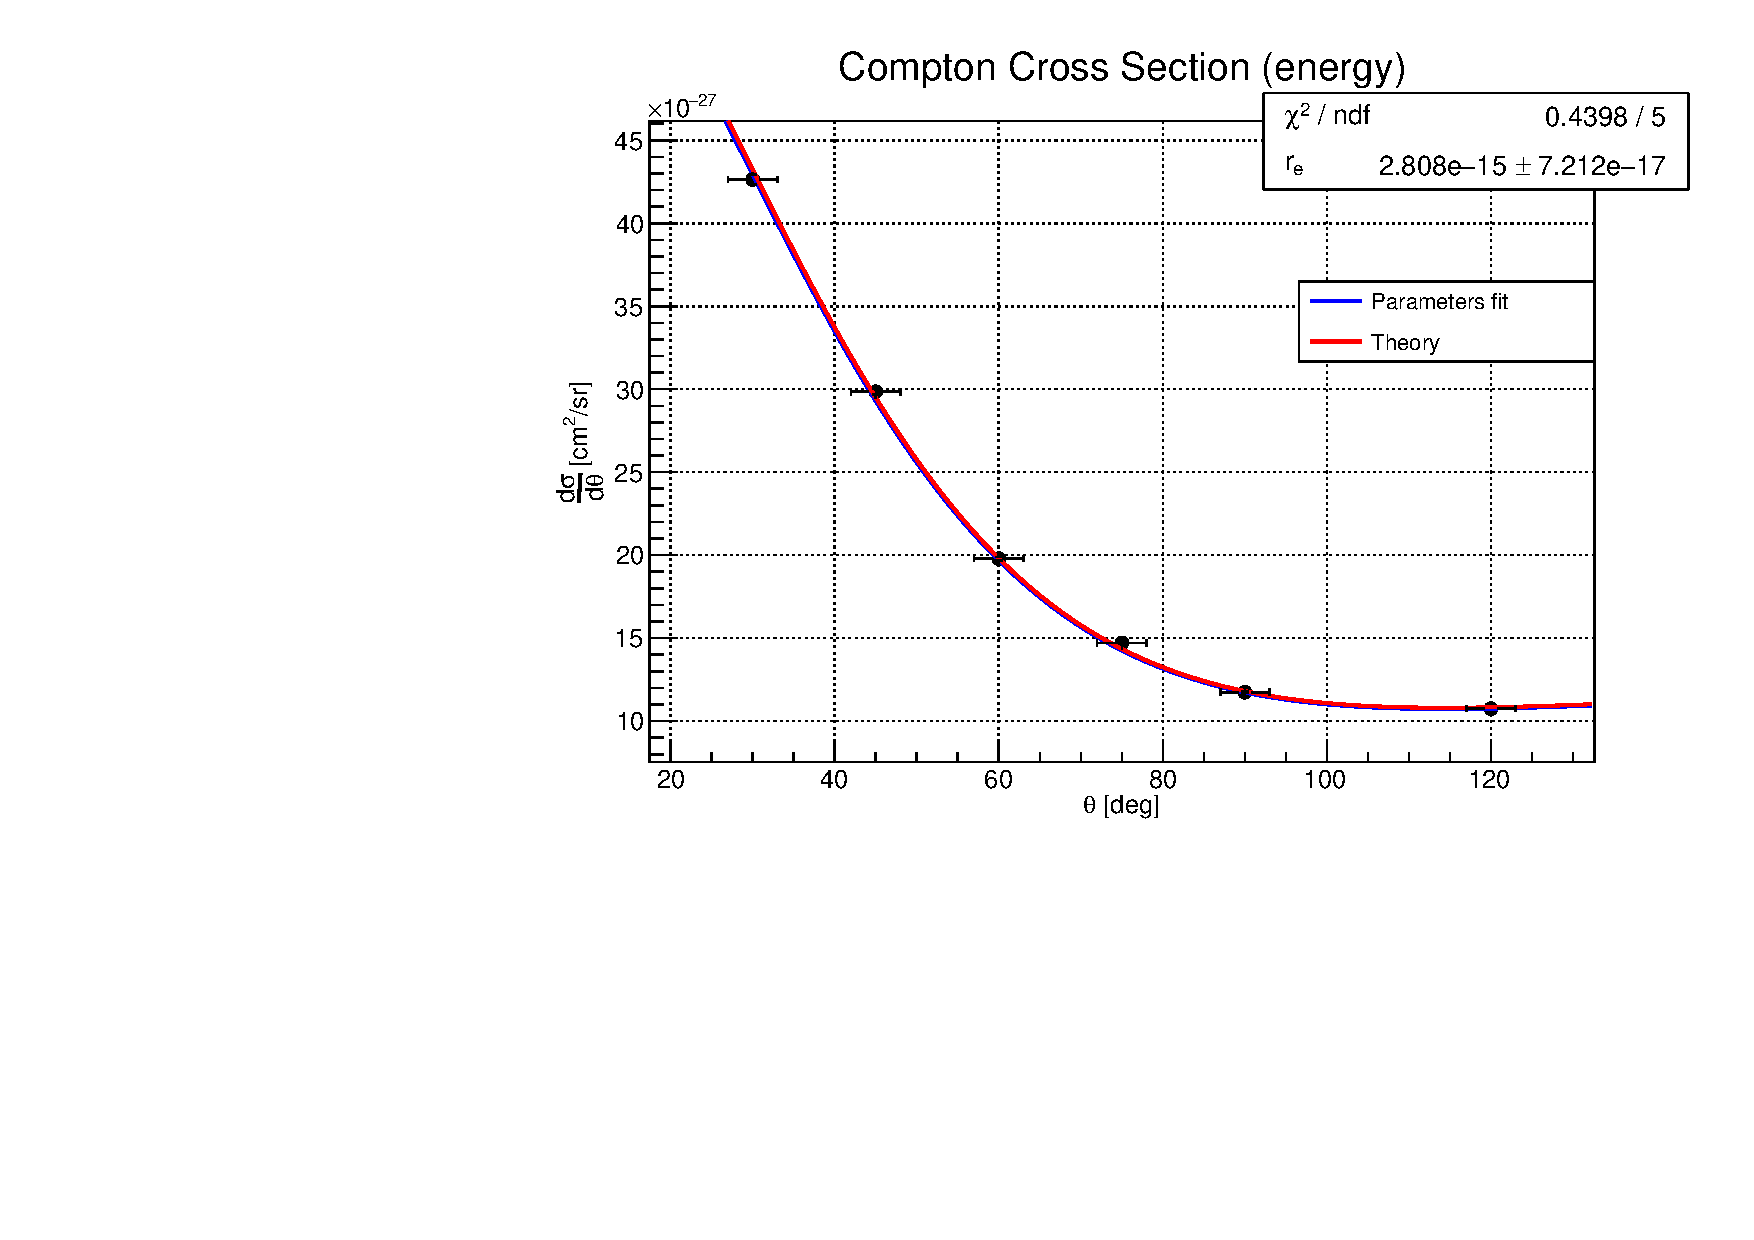
\includegraphics[scale=0.6]{Analisi Dati/ExpCrossSec_energy.pdf} 
  %\caption{Ricostruzione della sezione d'urto Compton tramite i picchi di energia}
  %\label{fig:sezione_energie}
%\end{figure}
%Analogamente a quanto fatto per i conteggi vi sono due fit che riproducono i seguenti risultati:
%\begin{table}[H]
   % \centering
   % \begin{tabular}{|c c c c c|}
   % \hline
   % Tipo di fit & $\chi^2$ & $ndf$ & Probabilità  & $r_e$ [fm]\\ [0.5ex] 
 %\hline\hline
 %Teorico & 7.99 & 6 & 24 \% & $\num{2.8179}$ \\ 
% \hline
% Parametrico & 0.439 & 5 & 99 \% & $\num{2.81}\pm\num{0.07}$\\ 
 %\hline 
 %   \end{tabular}
  %  \caption{Risultati di fit per la sezione d'urto Compton.}
    %\label{tab:risultati_sezione}
%\end{table}
%Si nota subito come le incertezze non siano visibili, in quanto nell'ordine di grandezza di $\num{e-28}\,\unit{\cm^{-2}}$ . Questo risulta dal fatto che le uniche incertezze coinvolte sono quelle relative ai picchi di energia e quella dell'angolo di scattering; quest'ultima in particolare risulta molto poco influente sul risultato.
%La stima del parametro $r_e$ risulta infine migliorata rispetto a quella precedente.

